\section{Intro and Motivation}
		Quantum spin liquids
		The Kitaev Honeycomb Model as the canonical QSL
		Anyons and braiding
		Non-abelian anyons
        What will be covered in this chapter
	
\section{Literature Review} 
\subsection{The Kitaev Honeycomb Model}

The Kitaev-Honeycomb model is remarkable because it was the first such model that combined three key properties.

First, it is a plausible tight binding Hamiltonian. The form of the Hamiltonian could be realised by a real material. Indeed candidate materials such as \ce{\alpha-RuCl3} were quickly found \cite{banerjeeProximateKitaevQuantum2016, trebstKitaevMaterials2022} that are expected to behave according to the Kitaev with small corrections. 

Second, the Kitaev Honeycomb model is deeply interesting to modern condensed matter theory. Its ground state is almost the canonical example of the long sought after quantum spin liquid state. Its excitations are anyons, particles that can only exist in two dimensions that break the normal fermion/boson dichotomy. Anyons have been the subject of much attention because, among other reasons, there are proposals to braid them through space and time to achieve noise tolerant quantum computations~\cite{freedmanTopologicalQuantumComputation2003}. 

Third and perhaps most importantly, it a rare many body interacting quantum system that can be treated analytically. It is exactly solveable meaning that we can explicitly write down its many body ground states in terms of single particle states~\cite{kitaevAnyonsExactlySolved2006}. Its solubility comes about because the model has extensively many conserved degrees of freedom that mediate the interactions between quantum degrees of freedom.

To get down to brass tacks, the Kitaev Honeycomb model is a model of interacting spin$-1/2$s on the vertices of a honeycomb lattice. Each bond in the lattice is assigned a label $\alpha \in \{ x, y, z\}$ and that bond couples its two spin neighbours along the $\alpha$ axis. 

This gives us the Hamiltonian
\begin{equation}
    \label{eqn:kitham}
    \mathcal{H} =  - \sum_{\langle j,k\rangle_\alpha} J^{\alpha}\sigma_j^{\alpha}\sigma_k^{\alpha},
\end{equation}
where $\sigma^\alpha_j$ is a Pauli matrix acting on site $j$, \(\langle j,k\rangle_\alpha\) is a pair of nearest-neighbour indices connected by an $\alpha$-bond with exchange coupling $J^\alpha$~\cite{kitaevAnyonsExactlySolved2006}.

% plaquette operators and wilson loops
This model has a set of conserved quantities that, in the spin language, take the form of Wilson loops 
\begin{equation}
W_p = \prod \sigma_j^{\alpha}\sigma_k^{\alpha}
\end{equation}
following any closed path of the lattice. In this product each pair of spins appears twice with two of the three bonds types, using the spin commutation relations we can replace each pair with the third. For a single hexagonal plaquette this looks like:
\begin{equation}
W_p = \sigma_1^{z}\sigma_2^{z} \sigma_2^{x}\sigma_3^{x} \sigma_3^{y}\sigma_4^{y} \sigma_4^{z}\sigma_5^{z} \sigma_5^{x}\sigma_6^{x} \sigma_6^{y}\sigma_1^{y}
\end{equation}
\begin{equation}
W_p = \sigma_1^{x}\sigma_2^{y} \sigma_3^{z} \sigma_4^{x} \sigma_5^{y}\sigma_6^{z}
\end{equation}
In this latter form can be seen to commute with all the terms in the Hamiltonian because {\color{red} why again?}

% relationship between wilson loops and topology
Such paths can enclose a collection of faces or `plaquettes' of the lattice. In the case of periodic boundary conditions, the system is torioidal and we also get Wilson loops that wind the whole system without enclosing a definite area. The loop operator associated with each such path has eigenvalues $/pm 1$ and can be interpreted as measuring the magnetic flux through that region. Without going into the details of counting them, the number of these conserved loop operators clearly scales with system size and it is this extensive number of classical degrees of freedom that ultimately allows us to decouple this interacting many body hamiltonian into a set of non interaction quadratic hamiltonians. {\color{red} add a figure showing the different kinds of Wilson loops and of an example plaquette}

% diagraom of a honeycomb lattice with majorana construction
\begin{figure}
    \centering
    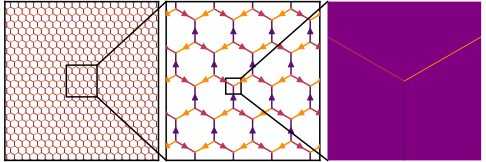
\includegraphics[width=\columnwidth]{figure_code/amk_chapter/honeycomb_zoom/intro_figure_template}
    \caption{\textbf{(a)} The standard Kitaev Model is defined on a honeycomb lattice. The special feature of the honeycomb lattice that makes the model solveable it is that each vertex is joined by exactly three bonds i.e the lattice is trivalent. One of three labels is assigned to each \textbf{(b)} We represent the antisymmetric gauge degree of freedom $u_{jk} = \pm 1$ with arrows that point in the direction $u_{jk} = +1$ \textbf{(c)} A visual analogy for The majorana transformation can be visualised as breaking each spin into}
    \label{fig:honeycomb_zoom}
\end{figure}

In order to actually solve the model we need to figure out how to leverage these conserved quantities. The trick is not so much a trick as an almost perfect consequence of the structure of the model and perhaps this was in fact how Kitaev first came up with it. We know that a single spin$-1/2$ can be represented by fermionic creation and annihilation operators $\sigma^{\pm} = 1/2(\sigma^x \pm \sigma^y)$ through a Jordan-Wigner transformation~\cite{}, this gives one fermion for each spin. In turn a fermion can be broken into two Majorana fermions $c_1 = 1/\sqrt{1}(f + f^\dagger)$ and $c_2 = i/\sqrt{1}(f - f^\dagger)$. If we double up the Hilbert space we get four Majoranas per spin: 

So how do we solve it? The trick is to replace each spin operator with 4 majorana operators (equivalent to two fermionic operators). 
 
The honeycomb lattice is bipartite, which means that it can be subdivided into two sub-lattices with only between sub-lattice couplings. It is also trivalent which means that each vertex connects to exactly three others. Finally, the edges of the lattice are three colourable, which means we can make an assignment (x,y,z) such that each site is connected to one of each type of edge. 

\subsection{Lattice generation}
% \begin{figure}
%     \centering
%     \includegraphics[width = \textwidth]{figs/pbc_voronoi.eps}
%     \caption{The construction of a periodic trivalent graph from a point set. The point set is replicated, a Voronoi transform is taken and finally the replication is undone. The graphs generated are trivalent except in very fine tuned cases which occur with low probability.}
%     \label{fig:pbc_voronoi}
% \end{figure}

We start from a set of points in the unit square. These can be drawn uniformly or via other methods such as using blue-noise or jammed circle packing. 

We then tile the plane with images of the point in the unit square and perform a voronisation over them. After this we can get rid of the images and relabel edges that cross the boundaries (red lines in fig \ref{fig:pbc_voronoi}) such that they connect points to the equivalent point within the unit cell.

We represent the graph structure with an ordered list of edges \((i,j)\) so we can represent both directed and undirected graphs which is useful for defining the sign of bond operators \(u_{ij} = - u_{ji}\).

% \subsetion{Kitaev-Heisenberg Model}
% In real materials there will generally be an addtional small Heisenberg term
% \begin{equation}
%     \label{eqn:kitaev_heisnberg}
%     \mathcal{H} =  - \sum_{\langle j,k\rangle_\alpha} J^{\alpha}\sigma_j^{\alpha}\sigma_k^{\alpha} + \sigma_j\sigma_k
% \end{equation}

% \section{The Projector} \label{apx:projector}
% {\color{red} Add brief mention of fermions and many body ground state}
% Closely following the derivation of~\cite{pedrocchiPhysicalSolutionsKitaev2011} we can extend to the amorphous case relatively simply. The main quantity needed is the product of the local projectors \(D_i\)
% \[\prod_i^{2N} D_i = \prod_i^{2N} b^x_i b^y_i b^z_i c_i \]
% for a lattice with \(2N\) vertices and \(3N\) edges. The operators can be ordered by bond type without utilising any property of the lattice.
% \[\prod_i^{2N} D_i = \prod_i^{2N} b^x_i \prod_i^{2N} b^y_i \prod_i^{2N} b^z_i \prod_i^{2N} c_i\]
% The product over \(c_i\) operators reduces to a determinant of the Q matrix and the fermion parity. The only problem is to compute the factors \(p_x,p_y,p_z = \pm1\) that arise from reordering the b operators such that pairs of vertices linked by the corresponding bonds are adjacent.
% \[\prod_i^{2N} b^\alpha_i = p_\alpha \prod_{(i,j)}b^\alpha_i b^\alpha_j\]
% This is simple the parity of the permutation from one ordering to the other and can be computed easily with a cycle decomposition.

% The final form is almost identical to the honeycomb case with the addition of the lattice structure factors \(p_x,p_y,p_z\)
% \[P^0 = 1 + p_x\;p_y\;p_z \mathrm{det}(Q^u) \; \hat{\pi} \; \prod_{\{i,j\}} -iu_{ij}\] 

% \(\mathrm{det}(Q^u)\) is the determinant of the matrix that takes \((c_1, c_2... c_{2N}) Q = (b_1, b_2... b_{2N})\). This along with \(\prod u_{ij}\) depend on the lattice and the particular vortex sector. 

% \(\hat{\pi} = \prod{i}^{N} (1 - 2\hat{n}_i)\) is the parity of the particular many body state determined by fermionic occupation numbers \(n_i\). The Hamiltonian is \(H = \sum \epsilon_i (n_i - 1/2)\) in this basis and this tells use that the ground state is either an empty system with all \(n_i = 0\) or a state with a single fermion in the lowest level. 



	        Conserved quantities -> plaquettes
			Majorana representation with 4 per site
			Alternative representation with with 3 majoranas per site
			Mapping to BdG hamiltonian
			Vortex defects and lattice defects
		    Kitaev on surfaces of genus g > 2

Plaquette Operators
Majorana representations
4 Majorana representation
3 Majorana representation
		    
\subsection{Amorphous Models}
			\subsection{The Weire-Thorpe Model}
			As a way to sanity check the code I was writing to work with the Kitaev Honeycomb Model on Amorphous lattices it was useful to reproduce some existing results. 
		
	

\section{The Amorphous Kitaev Honeycomb Model}
		Extending the kitaev honeycomb model to arbitrary trivalent lattices.
		Even and Odd Plaquettes
        Degeneracy and euler's equation

\begin{figure}
    \centering
    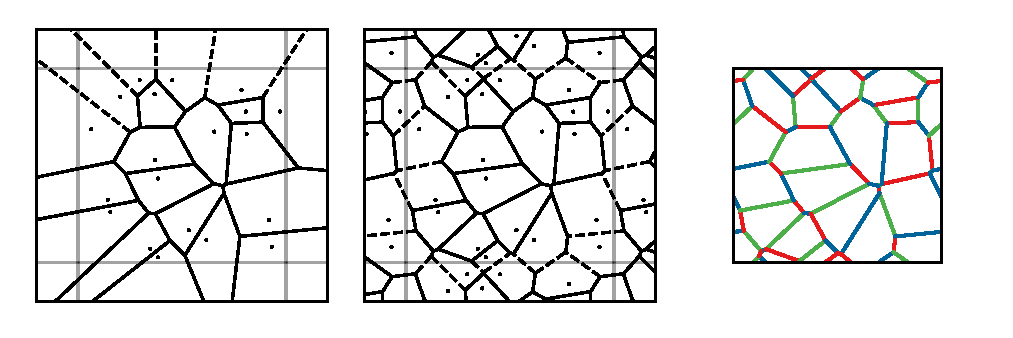
\includegraphics[width=\columnwidth]{figure_code/amk_chapter/lattice_construction/lattice_construction}
    \caption{\textbf{(a)} In-gap fermionic wavefunction drawn from the ground state flux sector in open boundary conditions, showing the state corresponds to a topological edge mode. Cut of the density along a line of lattice sites spanning the system (black line) is shown in the bottom subfigure on a logarithmic scale, demonstrating the characteristic exponential decay of topological edge modes with distance from the system edge. \textbf{(b)} Ground-state flux sector fermionic density of states in open boundary conditions, colored by inverse participation ratio. The increased inverse participation ratio of the in-gap states signifies their localisation to the edges of the system.}
    \label{fig:lattice_generation}
\end{figure}


\section{Methods}
        \subsection{Generating and Colouring Trivalent Graphs}
		\subsubsection{Voronisation}
		\subsubsection{Coloring}
		    The four colour theorem and its relation to edge colouring.
		    Finding Lattice colourings in practice: SAT solvers 
		
		\subsection{Finding the Ground State Flux Sector}
            A* star on the graph
		    Minimum spanning trees
    
\section{Results}
    \subsection{The Ground State}
	\section{Ground State Phase Diagram}
	\subsection{The Flux Gap}
	
		
\section{Conclusion}
\section{Discussion}
\section{Future Work}

\section{The Kitaev Honeycomb Model}

\subsection{The spin model}
The Kitaev-Honeycomb model is an exactly solveable model of interacting spins (or generic spin 1/2 degrees of freedom) on a honeycomb lattice. The Honeycomb lattice is bipartite and trivalent (each vertex connects to three others). The edges of the lattice are assigned to (x,y,z) such that each site is connected to one of each type of edge. 

\[H = \sum_{<i,j>} J_\alpha \sigma_i^{\alpha} \sigma_j^{\alpha} = \sum_{<i,j>} J_\alpha K_{ij}\]
where \(\alpha = \alpha(i,j)\) is the type of the bond linking sites i and j.

Various generalisations have been made, one mode replaces pairs of hexagons with heptagons and pentagons \cite{periNonAbelianChiralSpin2020} and another that replaces vertices of the hexagons with triangles \cite{yaoExactChiralSpin2007}. When we generalise this to the amorphous case, the key property that will remain is that each vertex interacts with exactly three others via an x, y and z edge. However the lattice will no longer be bipartite, breaking chiral symmetry among other things. 

The Hamiltonian commutes with the plaquette operators \(W_p\), products of the Ks around a plaquette. The Ks also commute with one another.
\[W_p = \prod_{<ij> \in P} K_{ij} = K_{12}K_{23}K_{34}K_{56} ... K_{N1}\]

Expanding the bond operators \(K_{ij} = \sigma_i^{\alpha} \sigma_j^{\alpha}\), Pauli operators on each site appear in adjacent pairs so can be replaced via \(\sigma_i \sigma_j = \delta_{ij} + \epsilon_{ijk} \sigma_k\) giving a product of Pauli matrices associated with the outward pointing bonds from the plaquette. In the general case:
\[W_p = \prod_{i \in P} i (-1)^{c_i} \sigma_i\]
where \(c_i = 0,1\) measures the handedness of the edges around vertex i, see Fig \ref{fig:handedness}. Plaquette operators for plaquettes with even numbers of edges square to 1 and hence have eigenvalues \(\pm 1\), while those around odd plaquettes have eigenvalues \(\pm i\) breaking chiral symmetry. The values of the plaquette operators partition the Hilbert space of the Hamiltonian into a set of flux sectors.


% \begin{figure}
%     \centering
%     \includegraphics[width = 0.5\textwidth]{figs/vertex_handedness}
%     \caption{Plaquette operators defined as a clockwise product of bond operators will contain a term \(...K_{ki}K_{ij}... = ...\sigma^\alpha_i \sigma^\beta_i ...\) which can be replaced with \(i (-1)^{c_i} \sigma_i^\gamma\) where \(c_i = 1\) if the bond types going clockwise around vertex i are a cyclic permutation of xyz otherwise \(c_i = 0\)}
%     \label{fig:handedness}
% \end{figure}

\subsection{A non-interacting Majorana representation}

The original Kitaev paper uses a transformation involving two fermionic modes per lattices site:
\[\acomm{f^\dagger}{f} = 1, \acomm{f}{f} = \acomm{f^\dagger}{f^\dagger} = 0\]
and the same for the second operator \(g\). They anti-commute with each other and the operators on other sites. It is also possible to transform to a Majorana basis with no redundant degrees of freedom \cite{fengTopologicalCharacterizationQuantum2007}.

We also have the number operators \(n_f = f^\dagger f\) and the total parity operator \(P = (2n_f - 1)(2n_g - 1)\) which divides the Hilbert space into even (\(\ket{00}, \ket{11}\)) and odd (\(\ket{01}, \ket{10}\)) parity subspaces. 

The Majorana modes are defined by:
\[b^x = f + f^\dagger\]
\[b^y = -i(f - f^\dagger)\]
\[b^z = g + g^\dagger\]
\[c = -i(g - g^\dagger)\]

Note that applying an odd number of Majorana operators to a state in one parity subspace will flip it to the other, while any even number preserves the parity subspace. 

The Pauli operators live in a two dimensional Hilbert space. We can build one from the fermionic subspace by projecting onto either the odd or even parity subspace defined above. The parity can be easily defined in terms of Majorana operators:

\[D = b^x b^y b^z c = - (2n_f - 1)(2n_g - 1) = - P\]

And the Pauli operators can be defined w.r.t states with D = 1 :
\[\sigma^\alpha = i b^\alpha c\]

With this choice, the Hamiltonian becomes quadratic:

\[H = \frac{i}{4} \sum_{<i,j>} 2 J_{\alpha_{ij}} u_{ij} c_i c_j\]
\[u_{ij} = i b^{\alpha_ij}_i b^{\alpha_ij}_j\]



\section{The Kitaev Honeycomb Model extended to an Amorphous Lattice}




\subsection{Edge Colouring}
% \begin{figure}
%     \centering
%     \includegraphics[width = .5\textwidth]{figs/dual_graphs.png}
%     \caption{Two graphs which are dual of one another.}
%     \label{fig:dual_graphs}
% \end{figure}

% \begin{figure}
%     \centering
%     \includegraphics[width = \textwidth]{figs/k5}
%     \caption{Embedings of the complete graph \(K_5\) and its dual \(D(K_5)\) onto the torus. The vertices of \(K_5\) cannot be 4 coloured and the edges of \(D(K_5)\) cannot be 3 coloured.}
%     \label{fig:k5}
% \end{figure}

Now that we have trivalent amorphous lattices, we need to assign \(\sigma_x, \sigma_y, \sigma_z\) to each edge. If we want the Majorana transformation to remain useful then we require that each site be connected to exactly on of each type of edge, otherwise the bond operators \(u_{ij}\) would not commute with one another and the model would not reduce to a quadratic form. This amounts to asking for a 3 coloring of the edges of the graph. 

The famous 4 colouring theorem proves that the vertices of all planar graphs can assigned one of four colors such that no neighbouring vertices share a colour using 4 colors or more. This can be turned into a proof that all trivalent planar graphs can be 3 edge coloured as follows:

1) Define the dual of a graph G to be D(G) such that plaquettes of G become vertices of D(G) and neighbouring plaquettes sharing an edge in D(G). It's easy to see that if G is planar then so is D(G). Note that each edge in G corresponds to an edge in D(G) and each vertex of G is surrounded by a triangle of three vertices in D(G).

2) The vertices of D(G) can be 4 coloured with colors (a,b,c,d)

3) Assign a color from (i,j,k) to the edges of D(G) (and thus to the edges of G) according to the colors of the vertices linked by the edge, ignoring ordering:

i if {a,b} or {c,d}
j if {a,c} or {b,d}
k if {a,d} or {b,c}

4) In a trivalent graph G, a vertex v in G is always part of 3 plaquettes (vertices in D(G)) and the colors of those plaquettes determines the colors of the edges that connect to v. The three vertices in D(G) must take three distinct colors from (a,b,c,d) so cannot lead to two edges with the same colour.

This implies that all trivalent planar graphs can have their edges 3 coloured. However we work in periodic boundary conditions and it's easy to embed the complete graph \(K_5\) into periodic boundary conditions, showing that the four colour theorem does not apply to periodic boundary conditions. However numerically we have not yet encountered even one case.

% \begin{figure}
%     \centering
%     \includegraphics[width = \textwidth]{figs/edge_color}
%     \caption{On the left, a single vertex in G, and the three dual-vertices in its dual D(G). If the dual-vertices of D(G) are 4 colored, the three dual-vertices shown must be three distinct colors, and hence if the colors of the edges in G are chosen according to the rules on the right, each will be distinct.}
%     \label{fig:edge_color}
% \end{figure}

\subsection{Finding Colourings}

Graph colouring is in NP, meaning that in general there is unlikely to be a polynomial time algorithm to compute it. However that does not mean that realistic instances of the problem are computationally intractable. A common method in computer science is to map NP problems onto a particular problem called Boolean Satisfiability for which general purpose and highly optimised solvers have been written.

The problems can be written as a a series of statements about a set of boolean variables, which we choose to be take to be the set \(l_{i\alpha}\) which indicate if edge i has colour \(\alpha\). We then have two types of contraint: each edge is exactly on colour and no neighbouring edges are the same color. 

I'll fill in the encoding later but the gist is that we can give this to a solver and get back: whether the problem is solveable, a solution or all the possible solutions. Finding a solution is relatively fast, while finding all the solutions is slower since there appear to be exponentially many of them. Fig \ref{fig:multiple_colourings} shows some examples. 


% \begin{figure}
%     \centering
%     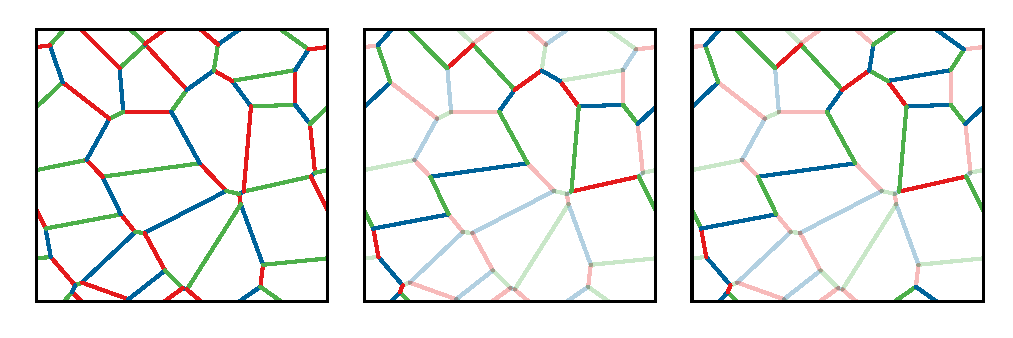
\includegraphics[width = \textwidth]{figs/multiple_colourings}
%     \caption{Multiple valid 3-edge-colourings of a random trivalent lattice. Edges are colored from red, green and blue and vertices are coloured red/blue if the edge colours are a cyclic/anticyclic permutation of rgb going clockwise around the vertex. Black edges or vertices indicate the color is the same as that in the top left. Note that some of the points are very close together, in future we will add a step to separate these.}
%     \label{fig:multiple_colourings}
% \end{figure}


\section{Weaire-Thorpe Models}
As a benchmark for our graph algorithms we reproduce results on the Weaire-Thorpe Model. The DOS agree very well but I haven't yet understood how to plot the edge states, plotting a single state in the gap or the sum of states in a finite energy region in the gap doesn't seem to look like an edge state.



% \begin{figure}
%     \centering
%     \includegraphics[width = \textwidth]{figs/WT_lattice}
%     \caption{An example of a Weaire-Thorpe model generated with our code.}
%     \label{fig:WT_lattice}
% \end{figure}

% \begin{figure}
%     \centering
%     \includegraphics[width = \textwidth]{figs/DOS_WT_Comp}
%     \caption{A comparison between the DOS from the paper (left) and the DOS generated using our code (right)}
%     \label{fig:DOS_WT_Comp}
% \end{figure}


\section{Open Questions}
\begin{itemize}
    \item Are the excitation spectra of the flux sectors disparate or overlapping?
    \item Will there be a qualitative difference between choosing +i for all plaquettes of odd length and of choosing +/-i so that they cancel out?
    \item
\end{itemize}

\section{The Projector}
Closely following the derivation given in~\cite{} we can extend the derivation of the projector to the amorphous case relatively simply. The final form is
\[P^0 = 1 + (-1)^{p_x + p_y + p_z} \left(-i \prod_{\{i,j\}} u_{ij}\right) \mathrm{det}(Q^u) \; \hat{\pi} \] 
where \(p_x,p_y,p_z\) are the parities of the permutations required to reorder the \(b^\alpha_i\) operators into an order where bonded sites are adjacent. These only depend on properties of the amorphous lattice used. In the HLM these terms can be computed analytically once a particular honeycomb lattice has been specified, we instead compute then numerically using a fast cycle decomposition algorithm.

\(\mathrm{det}(Q^u)\) is the determinant of the matrix that takes \((c_1, c_2... c_{2N}) Q = (b_1, b_2... b_{2N})\). This along with \(\prod u_{ij}\) depend on the lattice and the particular vortex sector. 

Finally \(\hat{\pi} = \prod{i}^{N} (1 - 2\hat{n}_i)\) is the parity of the particular many body state determined by fermionic occupation numbers \(n_i\). The Hamiltonian is \(H = \sum \epsilon_i (n_i - 1/2)\) in this basis and this tells use that the ground state is either an empty system with all \(n_i = 0\) or a state with a single fermion in the lowest level. 

\subsection{Derivation}
The projector is just a product of the site projectors, let's say there are \(2N\) sites.
\[D_i = b^x_i b^y_i b^z_i c_i \]
\[P = \prod_i^{2N} (1 + D_i)\]

The clever trick from \ref{} is to note that this corresponds to a sum over products of all possible subsets of the integers (the powerset) of our 2N \(D_i\) operators. 

If we think of these subsets as bitstrings of length \(2N\) the we can write this as a sum over integers \(n\) where \(n_i = 0,1\) is the ith bit of \(n\).
\[P = \sum_{n = 0}^{2^{2N}} \prod_{i=0}^{2N} D_i^{n_i}\]

then the ``all ones'' operator \(F = \prod_i D_i\) acts as the bitwise not operation on any other subset:
\[ \prod_i D_i \prod_{i=0}^{2N} D_i^{n_i} = \prod_{i=0}^{2N} D_i^{1 - n_i}\]
Hence we can actually just sum over half the integers and use this operator to get the other half:
\[P = \left(\sum_{n = 0}^{2^{2N - 1}} \prod_{i=0}^{2N} D_i^{n_i} \right) (1 + \prod_{i=0}^{2N} D_i) = S P^0\]

The paper argues that S will never give zero on any state for reasons I do not understand, though one can make an argument that since \(P^0\) already removes half the states from the Hilbert space, S cannot remove anymore.  We therefore focus on computing \(P^0\).

\[\prod_{i=1}^{2N} D_i = b^x_1 b^y_1 b^z_1 c_1\; b^x_2 b^y_2 b^z_2 c_2\; ... \;b^x_{2N} b^y_{2N} b^z_{2N} c_{2N}\]

We can move all the \(c_i\) operators to the right, incurring \(3(i-1)\) swaps for each giving a factor of \(-1 ^ \theta_c\) where \( \theta_c = {3N(2N-1)} = \sum{i = 1}^{2N} 3(i-1)\)

\[\prod_{i=1}^{2N} D_i = -1^{\theta_c}b^x_1 b^y_1 b^z_1\; b^x_2 b^y_2 b^z_2\; ... \;b^x_{2N} b^y_{2N} b^z_{2N}\;\prod_{i=1}^{2N}c_i\]

All the \(b^x\) terms are separated by pair other operators so can be brought to the front with no additional factors.

\[\prod_{i=1}^{2N} D_i = -1^{\theta_c}\left(\prod_{i=1}^{2N}b^x_i\right) b^y_1 b^z_1\; b^y_2 b^z_2\; ... \; b^y_{2N} b^z_{2N}\;\left(\prod_{i=1}^{2N}c_i\right)\]

Finally we can send each \(b^z_i\) to the right incurring \(i\) swaps giving \(\theta_z = N(2N - 1)\) 

How to do open boundary conditions

Note: we don't actually compute \(p_x\) we compute \(-1ˆp_x\) directly using a cycle decomposition to compute the permutation parity.


    
    
    